\documentclass[tikz, border=20pt]{standalone}
\usepackage{xcolor}
\usepackage{tikz}
\usetikzlibrary{arrows.meta, positioning, fit, backgrounds, shapes.misc, matrix, calc}

\definecolor{svlcolor0}{HTML}{F0F0F0}
\definecolor{svlcolor1}{HTML}{000000}
\definecolor{svlcolor2}{HTML}{FFD700}
\definecolor{svlcolor3}{HTML}{90EE90}
\tikzset{
  code_line/.style={anchor=west, font=\ttfamily},
  code_highlight/.style={code_line, fill=yellow!20, rounded corners=2pt, inner sep=2pt},
  element_idle/.style={draw=black!60, fill=black!10, minimum size=1cm, line width=1pt, rounded corners=2pt},
  element_idle_node/.style={circle, draw=black!60, fill=black!10, minimum size=1.0cm, line width=1pt, align=center, font=\small},
  element_current_node/.style={element_idle_node, fill=yellow!30},
  element_default/.style={element_idle},
  edge_normal_edge/.style={line width=1.2pt, color=black!60, shorten >=2pt, shorten <=2pt},
  edge_tree_edge/.style={edge_normal_edge},
  cell_current_cell/.style={fill=yellow!20, rounded corners=1pt},
  box_default_boundary/.style={draw=black!50, dashed, rounded corners=3pt, inner sep=8pt},
  dep_arrow/.style={color=red!70, line width=1pt, ->, >=Stealth},
  comment_default_comment/.style={draw=black!30, fill=white, rounded corners=2pt, inner sep=2pt},
  element_idle/.style={draw=black!60, fill=svlcolor0, text=svlcolor1, minimum size=1cm, line width=1pt, rounded corners=2pt},
  cell_idle/.style={fill=svlcolor0, draw=black!60, rounded corners=1pt},
  element_comparing/.style={draw=black!60, fill=svlcolor2, text=svlcolor1, minimum size=1cm, line width=1pt, rounded corners=2pt},
  cell_comparing/.style={fill=svlcolor2, draw=black!60, rounded corners=1pt},
  element_swapped/.style={draw=black!60, fill=svlcolor3, text=svlcolor1, minimum size=1cm, line width=1pt, rounded corners=2pt},
  cell_swapped/.style={fill=svlcolor3, draw=black!60, rounded corners=1pt},
  edge_idle/.style={line width=1.5pt, color=black!60, shorten >=2pt, shorten <=2pt},
  dep_idle/.style={color=black!60, line width=1.5pt, ->, >=Stealth},
  edge_comparing/.style={line width=1.5pt, color=black!60, shorten >=2pt, shorten <=2pt},
  dep_comparing/.style={color=black!60, line width=1.5pt, ->, >=Stealth},
  edge_swapped/.style={line width=1.5pt, color=black!60, shorten >=2pt, shorten <=2pt},
  dep_swapped/.style={color=black!60, line width=1.5pt, ->, >=Stealth},
  cell_changed/.style={fill=yellow!25, rounded corners=1pt}
}
\begin{document}
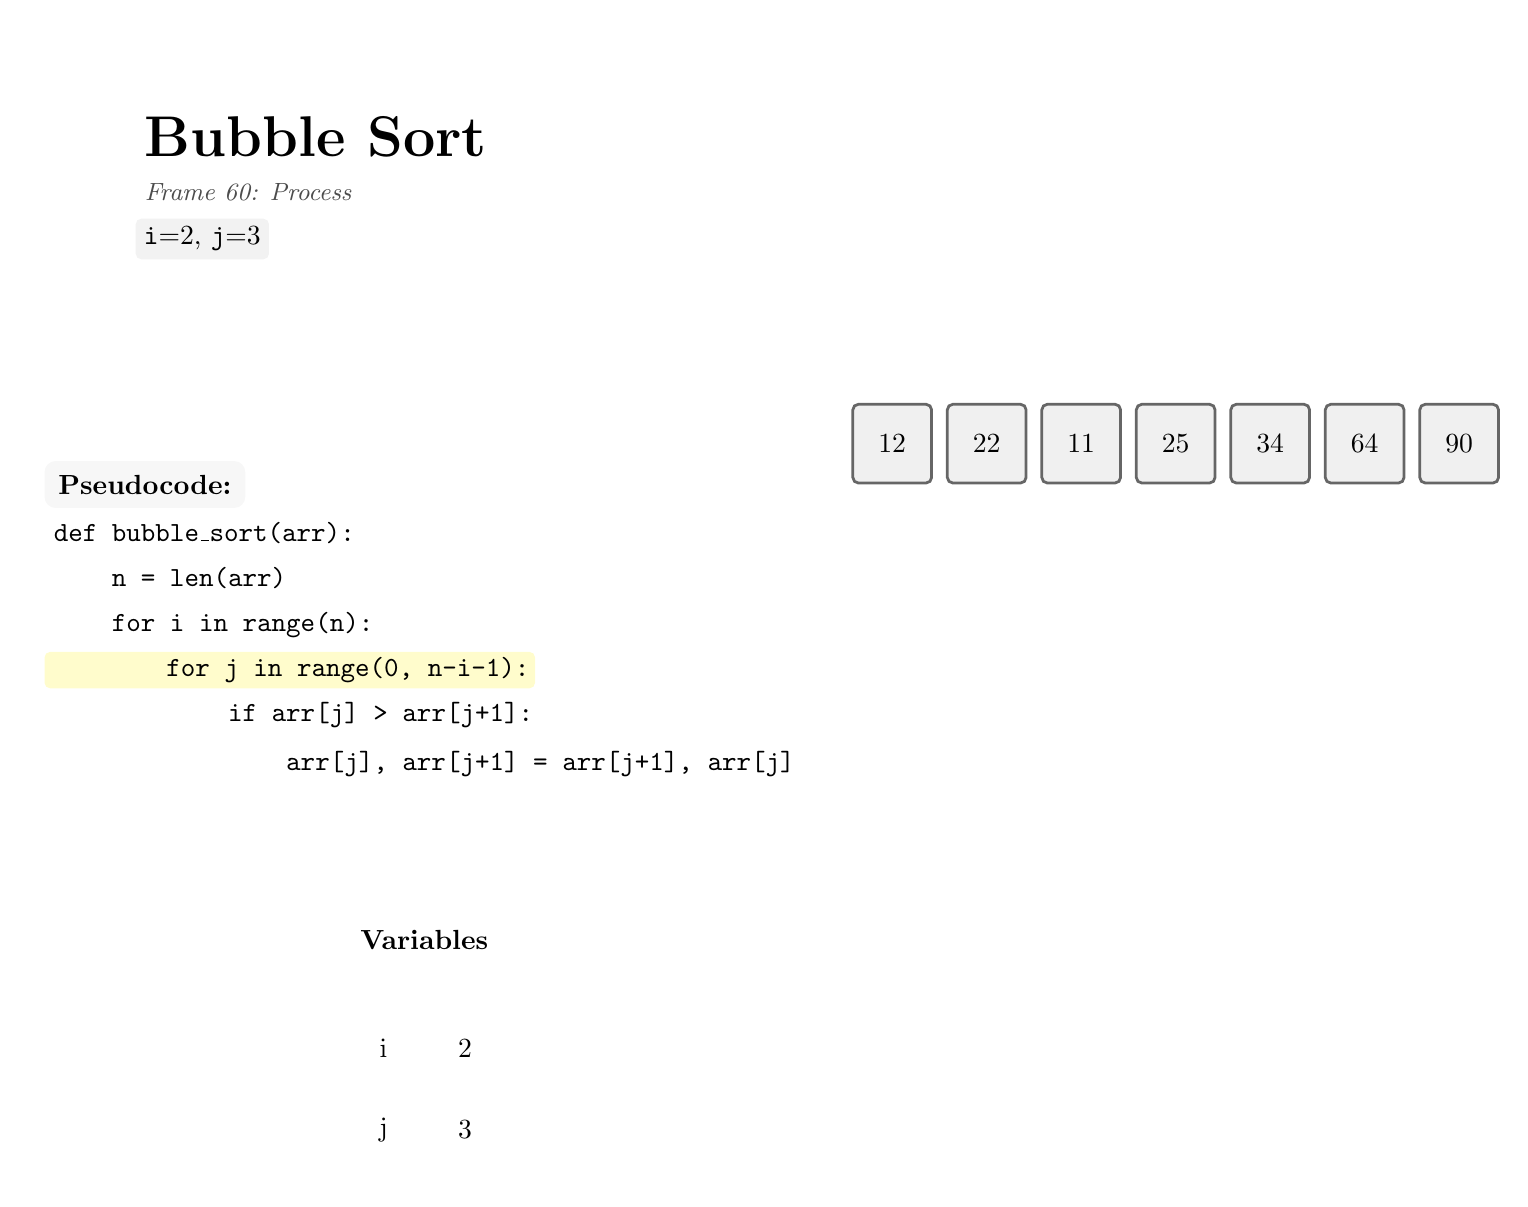
\begin{tikzpicture}[x=1cm, y=1cm, every node/.style={transform shape}]
\path (0, 1.0) -- (0, 0);
\node[font=\huge\bfseries, anchor=north west] (title_node) at (0,0) {Bubble Sort};
\node[font=\small\itshape, color=black!70, below=0.1cm of title_node.south west, anchor=north west] (subtitle_node) {Frame 60: Process};
\node[font=\normalsize, fill=black!5, rounded corners=2pt, inner sep=3pt, below=0.1cm of subtitle_node.south west, anchor=north west] (vars_node) {\texttt{i}=2, \texttt{j}=3};
\node (left_col_start) [below=0.8cm of vars_node.south west, anchor=north west] {};
\node[font=\bfseries, anchor=west, fill=black!3, rounded corners, inner sep=5pt] (pseudo_title) [below=1.5cm of left_col_start, anchor=north] {Pseudocode:};
\node[code_line, font=\ttfamily, anchor=north west] (pseudo_line_0) at ($(pseudo_title.south west) + (0, -0.05)$) {\hspace*{0.0em}def bubble\_sort(arr):};
\node[code_line, font=\ttfamily, anchor=north west] (pseudo_line_1) at ($(pseudo_line_0.south west) + (0, -0.05)$) {\hspace*{2.0em}n = len(arr)};
\node[code_line, font=\ttfamily, anchor=north west] (pseudo_line_2) at ($(pseudo_line_1.south west) + (0, -0.05)$) {\hspace*{2.0em}for i in range(n):};
\node[code_highlight, font=\ttfamily, anchor=north west] (pseudo_line_3) at ($(pseudo_line_2.south west) + (0, -0.05)$) {\hspace*{4.0em}for j in range(0, n-i-1):};
\node[code_line, font=\ttfamily, anchor=north west] (pseudo_line_4) at ($(pseudo_line_3.south west) + (0, -0.05)$) {\hspace*{6.0em}if arr[j] > arr[j+1]:};
\node[code_line, font=\ttfamily, anchor=north west] (pseudo_line_5) at ($(pseudo_line_4.south west) + (0, -0.05)$) {\hspace*{8.0em}arr[j], arr[j+1] = arr[j+1], arr[j]};
\node[fit=(pseudo_title) (pseudo_line_0) (pseudo_line_1) (pseudo_line_2) (pseudo_line_3) (pseudo_line_4) (pseudo_line_5), inner sep=0.2cm] (pseudo_block) {};
\node[font=\bfseries, below=1.5cm of pseudo_block] (title_vars_panel) {Variables};
\matrix (matrix_vars_panel) [below=0.5cm of title_vars_panel, matrix of nodes, nodes={minimum size=1.0cm, anchor=center}, column sep=1pt, row sep=1pt] {
i & 2 \\
j & 3 \\
};
\node[fit=(title_vars_panel) (matrix_vars_panel-1-1), inner sep=0.1cm] (aux_view_block_0) {};
\node[fit=(title_vars_panel) (matrix_vars_panel-1-1), inner sep=0.1cm] (first_aux_view_block) {};
\node[fit=(title_vars_panel) (matrix_vars_panel-1-1), inner sep=0.1cm] (last_aux_view_block) {};
\node[fit={(first_aux_view_block) (last_aux_view_block)}, inner sep=0.1cm] (aux_full_block) {};
\node[fit={(pseudo_block) (aux_full_block)}, inner sep=0pt] (left_column_box) {};
\node (right_col_start) at ($(left_column_box.north east) + (4.5cm, 0)$) {};
\begin{scope}[shift={($(right_col_start) + (0, 0.0)$)}]
\node[element_idle] (a0) at (-3.5999999999999996, 0.0) {12};
\node[element_idle] (a1) at (-2.3999999999999995, 0.0) {22};
\node[element_idle] (a2) at (-1.1999999999999997, 0.0) {11};
\node[element_idle] (a3) at (0.0, 0.0) {25};
\node[element_idle] (a4) at (1.2000000000000002, 0.0) {34};
\node[element_idle] (a5) at (2.4000000000000004, 0.0) {64};
\node[element_idle] (a6) at (3.5999999999999996, 0.0) {90};
\end{scope}
\path (title_node.north west) -- (current bounding box.south east);
\end{tikzpicture}
\end{document}
